\section{The Advanced Encryption Standard (AES)}

On September 12, 1997, the United States' National Institute of
Standards and Technology (NIST) announced an open competition to
develop a new symmetric-key block cipher algorithm to replace the
ageing DES (Data Encryption Standard). The demands was that the AES
should be an unclassified, public, and royalty-free symmetric-key
encryption algorithm supporting block sizes of 128-bits, key sizes of
128-, 192- and 256-bits.

On October 2, 2000, NIST announced that it had selected
Rijandael~\cite{rijandael}, designed by two Belgium cryptographers:
Daemen and Rijmen, as the AES.

%As of today, multiple processors include native support for
%acceleration of AES-specific operations. NIST has also called for the
%development of a new hash-function, and 4 of 14 of the remaining
%candidates rely on native AES-acceleration to acheive performance.

\subsection{Overview of the algorithm}

Rijandael is a symmetric-key block-cipher algorithm. This means that
encryption is defined as $c \leftarrow E_k(m)$, and decryption as $m
\leftarrow D_k(c)$, given a key $k$, a message $m$ and a ciphertext
$c$. Rijandael supports variouskey sizes, but I will confine the
description and implementation to a key size to
\unit{128}{\bit}. This will not cause a big loss of generality to the
working principle. I will also limit the implementation to
encryption-only.

The Rijandael cipher segments a 128-bit message into 16 bytes,
represented by a $4 \times 4$ matrix:

\begin{equation}
  m = \begin{pmatrix}
    m_0 & m_4 & m_8 & m_{12} \\
    m_1 & m_5 & m_9 & m_{13} \\
    m_2 & m_6 & m_{10} & m_{14} \\
    m_3 & m_7 & m_{11} & m_{15}
    \end{pmatrix}
\end{equation}

This is referred to as the $State$ throughout the algorithm, and it is
permutated 10 $Round$s in the algorithm. For larger key sizes, the
number of rounds should be increased. A round is composed of four
transformations described below:

\begin{eqnarray*}
&Round&(State, RoundKey) \{\\
  & &SubBytes (State)\\
  & &ShiftRows (State)\\
  & &MixColumns (State)\\
  & &AddRoundKey (State, RoundKey)\\
&\}&
\end{eqnarray*}

The final round, $FinalRound$, is slightly different: it excludes the
MixColumns stage. $RoundKey$ is derived from the key by the key
expansion scheme also described below. For decrypting, given the
correct key, there exists inverse functions for each round.

The Rijandael cipher work in a finite field. The field is realized as
all polynomials modulo the irreductible polynomial 
\begin{equation}
  f(x) = x^8 + x^4 + x^3 + x + 1
  \label{eq:gf}
\end{equation} 
over $\mathbb{F}_2$. This is called the ``Rijandael
field'', and $\mathbb{F}_{2^8}$ is often used to denote the field with
256 elements.

Each element can also uniquely be represented as a 8-bit byte, $\{b_7
b_6 b_5 b_4 b_3 b_2 b_1 b_0\}$ yielding the polynomial $\sum_{i=0}^7
b_i x^i$, where $b_i \in \mathbb{F}_2$ where $\mathbb{F}_2 =
\{0,1\}$. The polynomial $x^2 + 1$ can thereby be represented as
$\{00000101\}$, or hexadecimaly as $\{05\}$.  All operations on
elements in this field results in an element within the field. The
field supports addition and multiplication between two field elements.

The $SubBytes$ routing subtitutes all bytes using $y = A x^{-1} + b$.
%%  where $
%%   A =
%%   \begin{pmatrix}
%%     1 & 0 & 0 & 0 & 1 & 1 & 1 & 1 \\
%%     1 & 1 & 0 & 0 & 0 & 1 & 1 & 1 \\
%%     1 & 1 & 1 & 0 & 0 & 0 & 1 & 1 \\
%%     1 & 1 & 1 & 1 & 0 & 0 & 0 & 1 \\
%%     1 & 1 & 1 & 1 & 1 & 0 & 0 & 0 \\
%%     0 & 1 & 1 & 1 & 1 & 1 & 0 & 0 \\
%%     0 & 0 & 1 & 1 & 1 & 1 & 1 & 0 \\
%%     0 & 0 & 0 & 1 & 1 & 1 & 1 & 1
%%   \end{pmatrix}$ and $
%%   b = 
%%   \begin{pmatrix}
%%     1\\1\\0\\0\\0\\1\\1\\0
%%   \end{pmatrix}$.
That is, inversion in the finite galois field, followed by a short
linear transformation.

$ShiftRows$ is a permutation of the order of the bytes in the state:
\begin{equation}
  \begin{pmatrix}
    s_0 & s_4 & s_8    & s_{12} \\
    s_1 & s_5 & s_9    & s_{13} \\
    s_2 & s_6 & s_{10} & s_{14} \\
    s_3 & s_7 & s_{11} & s_{15}
  \end{pmatrix} 
  \rightarrow
  \begin{pmatrix}
    s_0    & s_4    & s_8    & s_{12} \\
    s_{13} & s_1    & s_5    & s_9 \\
    s_{10} & s_{14} & s_2    & s_6 \\
    s_7    & s_{11} & s_{15} & s_3    
    \end{pmatrix}
\end{equation}
In VLSI circuits, this is easily implemented as wiring.

The $MixColumn$ procedure scrambles all the columns in the state
%given as $
%\begin{pmatrix}
%  s_0\\s_1\\s_2\\s_3
%\end{pmatrix}$, 
by multiplying them with the matrix
\begin{equation}
  \begin{pmatrix}
    \{02\} & \{03\} & \{01\} & \{01\} \\
    \{01\} & \{02\} & \{03\} & \{01\} \\
    \{01\} & \{01\} & \{02\} & \{03\} \\
    \{03\} & \{01\} & \{01\} & \{02\}
  \end{pmatrix}
  \label{eq:mixcol}
\end{equation}
in the galois field. Multiplication, $q(x)=a(x) \otimes b(x)$, in the
galois field is multiplication of two polonomials modulo the
irreductible polinomial \eqref{eq:gf}. The multiplication can be
performed by generating up to eight partial products
\begin{equation}
  P_i(x) = a(x) x^i
\end{equation}
iterativly as 
\begin{equation} 
  P_i = 
  \begin{cases}
    a(x) & \text{if} \quad i = 0 \\
    x P_{i-1}(x) & \text{if} \quad i > 0
  \end{cases}
  \label{eq:gfdouble}
\end{equation}
and then adding the partial products according to the bits $b_i$ in
$b(x)$, yielding the result as
\begin{equation}
  q(x) = \sum_{i=0}^{7} P_i(x) b_i
  \label{eq:addpart}
\end{equation}
. Note that the $\sum$ here performs the additions in the Galois
field, i.e. it sums with xor. Each iteration with $i > 0$ in
\eqref{eq:gfdouble} can be seen as a ``doubling'' in the galois field,
making the multiplication an analogy to peasant's multiplication in
\eqref{eq:addpart}. The ``doubling'' can be implemented with a shift
and 3 xor gates.

$AddRoundKey$ performs simple addition of the expanded key and the
state in the galois field. This addition can be implemented by simple
xor. The expanded key, derived from the input key, is calculated by
operations similar to the round function, and needs 4 bytes of
$SubBytes$ transformation as well.

\subsection{Performance of the AES}

As a reference of the relative performance of the AES, a simple
benchmark was done on a computer\footnote{openssl version
  0.9.8g. Measurement performed with the command ``openssl time
  aes''.}. The results are shown in table~\ref{tab:aes}. A feasability
study \cite{feas} shows that througput up to \unit{500}{\giga \bit
  \per \second} should be possible on VLSI.

\begin{table}[h]
  \centering
  \begin{tabular}{|c|c|}
    \hline
    \emph{Key size}  & \emph{Throughput} \\ \hline
    \unit{128}{\bit} & \unit{111}{\mega \byte \per \second} \\
    \unit{192}{\bit} & \unit{94.7}{\mega \byte \per \second} \\
    \unit{256}{\bit} & \unit{82.3}{\mega \byte \per \second} \\ \hline
  \end{tabular}
  \caption{Performance of AES on an Intel Pentium 4 2.8 GHz CPU.}
  \label{tab:aes}
\end{table}

The clockless AES module designed in \cite{claes}, which did not have
performance as a primary objective, performed \unit{283.75}{\kilo
  \byte \per \second} on \unit{0.35}{\micro \meter} CMOS.

\subsection{Details for VLSI implementation}

When implementing AES to hardware, there are a lot of choices and
optimizations that can be applied. I will here outline some aspects of
implementing AES. More methods for saving power and enhancing
performance are rigourously surveyed in \cite{ekelund}.

Naivly, the $SubBytes$ routine and its inverse is implemented with a
table lookup with 256 entries. In hardware, this means some kind of a
ROM, with an unbreakable latency and the inherent impossibility for
pipelining. In \cite{csbox} a method is described for decomposing the
$2^8$ fields into smaller $2^4$ fields for calculating the
multiplicative inverse combinationally.

The AES algorithm in itself is considered a secure cipher, that is, no
other methods other than brute-force attacks exists to deduce a key or
plaintext. However, an implementation of AES in software or hardware
can be subject to side-band attacks. If an attacker has physical
access to a weak system performing AES, multiple techniques exists for
retrieving information about the key.

If not careful implemented, a circuit can exhibit non-constant timing
when performing, revealing patterns of the data being processed, that
being the key or plaintext. Implementations can also have weaknesses
where the power dissipation depends on the data, which lets a careful
attacker measure and gather data about the key. A third method is to
inject faults into a system, making it malfunction and reveal secret
data.

The clockless AES implemented in \cite{claes} was developed to avoid
these kind of attacks, and concludes that their dual-rail
implementation hides the secret data from power, timing and
fault-injection attacks. It is worth to note that the ROM-based
implementation of $SubBytes$ that was utilized in this implementation
showed major leaks of information in the circuit. Side-band
information is leaked as a consequence of different hamming-weights
are giving different power signatures, and this problem is alleviated
in \cite{claes} by employing dual-rail encoding, ensuring constant
hamming-weight at the electrical level for all data.

\subsection{Pipelining and mode of operation}

While it is possible to pipeline the $Round$ procedure by itself, and
even $SubBytes$ itself when implemented combinationally as in
\cite{csbox}, it can also be beneficial to unroll multiple $Round$s in
series. I will here describe 3 modes of operation to illustrate when
unrolling can be beneficial.

\begin{figure}[htbb]
  \subfigure{\label{fig:ecbpicta}}
  
\includegraphics[width=0.3\textwidth]{tux.jpeg}
  \subfigure{\label{fig:ecbpictb}}
  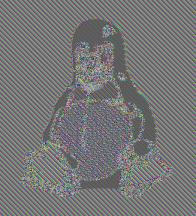
\includegraphics[width=0.3\textwidth]{tux_ecb.jpeg}
  \subfigure{\label{fig:ecbpictc}}
  
\includegraphics[width=0.3\textwidth]{noise.png}
  \caption{a) A picture encrypted in b) ECB-mode and in c) other
    modes, causing an unrevealing pseudo random pattern. Figure from
    \cite{pingu}.}
  \label{fig:ecbpict}
\end{figure}

When encrypting a plaintext with a length over 128 bits, the most
straightforward way is to split the plaintext into 128-bit blocks and
encrypt them individually. This is called the electronic codebook mode
of operation, or ECB. As the blocks can be encrypted and decrypted
independently, this method allows pipelining with unrolled
$Round$s. However, as the AES-algorithm deterministicly yields the
same output given the same input (key and data), it allows an attacker
to guess the ciphertext by trial-and-error. Figure~\ref{fig:ecbpict}
illustrates how ECB reveals data-patterns from the plaintext.


\begin{figure}[htbb]
  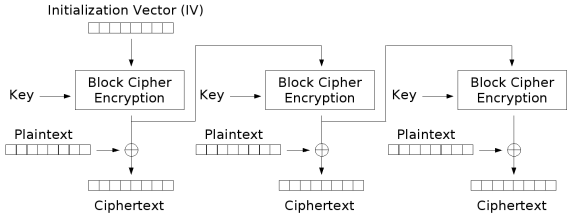
\includegraphics{ofb.png}
  \caption{Output feedback (OFB) mode encryption. Figure from \cite{pingu}.}
  \label{fig:ofb}
\end{figure}

The output feedback (OFB\nomenclature{OFB}{Output Feedback}) mode of
operation, described in figure~\ref{fig:ofb}, while not suffering from
the same weakness as the ECB\nomenclature{ECB}{Electronic Code Book}
mode, does not benefit from unrolling, as the preceeding ciphertext is
needed to encrypt the current plaintext. The OFB mode generates a
pseudo random (but unguessable, not given the key) string that is
XORed\nomenclature{XOR}{Exclusive OR} with the plaintext to encrypt,
similar to the Vernam one-time-pad cipher \cite{vernam}.

The only mode of operation considered secure, to my knowledge, that
benefit from loop unrolling, is the counter
(CTR)\nomenclature{CTR}{Counter} mode. In this mode, similar to the
OFB mode, a pseudorandom string is generated simpy by encrypting an
integer, $i$, corresponding to the current block number, that is $c_i
= m_i \oplus E_k(i)$, and similarily $m_i = c_i \oplus E_k(i)$, where
$\oplus$ denotes XOR. Whithout feedback, the CTR mode allows random
access during encryption and decryption (for e.g. full disk
encryption), and blocks can be processed in paralell.

\subsection{Decryption and other keysizes}

While this project does not cover decryption and the larger keysizes,
that is 192 and 256 bit, I will shortly outline how this can be
implemented, and roughly estimate the impact on area and performance
it will inflict.

The decryption is rougly the algorithms performed inversely with
reverse operations for $SubBytes$, $ShiftRows$, $MixColumns$ and
$AddKey$: 
\begin{itemize}
  \item $SubBytes^{-1}$, implemented combinationally, is the same
    operation as $SubBytes$, except for the relativily short linear
    transform, which needs an inverse. 
  \item $ShiftRows^{-1}$ has, like $ShiftRows$, the simplest
    implementation as wires. 
  \item $MixColumns^{-1}$ uses different and larger coefficients
    than $MixColumns$ \eqref{eq:mixcol}, demanding 2 more partial
    products \eqref{eq:gfdouble} to be calculated in the
    galois field multiplications, and thereby causing longer
    delays. The calculation of the partial products can be shared
    between $MixColumns$ and its inverses. 
  \item $AddRoundKey^{-1}$ can use the same hardware as
    $AddRoundKey$. 
\end{itemize}
The keyschedule for the decryption is the same as for encryption.

Expanding the algorithm to key sizes of 192 and 256 bit requires
expansion of the key registers and changes to the control logic and
the key schedule. The control logic must be changed, as 128, 192, and
256 bit keys respectivily requires 10, 12, and 14 $Round$s to be
performed. The key schedule also demands an extension of the control
logic to support the larger key sizes.

Implementing decryption alongside with encryption will, as discussed
above, have negative effect on the performance, as there will be a
greater control overhead. The area will also increase, but as most of
the operations can be generalized to also provide an inverse, the area
overhead should not be dramatic. Expansion of the supported key sizes,
in addition to the obvious demand of larger registers, only requires
minor expansion of the control logic.
